\begin{tabular}{ccc}
    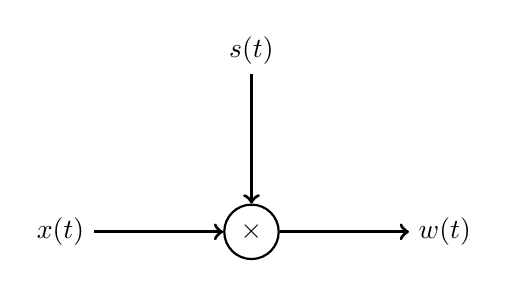
\begin{tikzpicture}
    \node[circle,radius=1cm,draw,thick] (x) at (0,0) {$\times$};
    \node[above=2cm] (deltatrain) at (x) {$s(t)$};
    \node[left=2cm] (x_t) at (x) {$x(t)$} ;
    % \node[right=1.5cm,rectangle,draw,thick,inner sep=0.5cm] (H_jw) at (x) {$H(j\omega)$} ;
    % \node[right=2cm] (x_r) at (H_jw) {$y(t)$} ;
    \node[right=2cm] (w) at (x) {$w(t)$} ;
    
    \draw[->,very thick] (deltatrain) -- (x) ;
    \draw[->,very thick] (x_t) -- (x) ;
    \draw[->,very thick] (x) -- (w) ;
    % \draw[->,very thick] (x) -- (H_jw) ;
    % \draw[->,very thick] (H_jw) -- (x_r) ;
    \end{tikzpicture} & \hfill &
    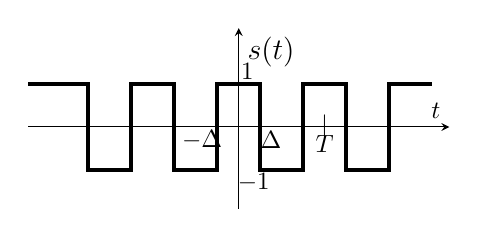
\begin{tikzpicture}[scale=0.9,transform shape]
    \begin{axis}[
        x=0.05\textwidth,y=0.05\textwidth,
        axis y line=center,
        axis x line=middle,
        xlabel=$t$,ylabel={\large $s(t)$},
        xmin=-4.9,xmax=4.9,
        ymin=-1.9,ymax=2.3,
        ticks=none
        ]
        \addplot[
        black,
        ultra thick
        ] coordinates {
            (-5.5,1) (-4.5 1) (-3.5, 1) (-3.5,-1) (-2.5,-1) (-2.5, 1) (-1.5, 1) (-1.5, -1) (-.5,-1) (-.5,1) (.5,1) (.5,-1) (1.5,-1) (1.5,1) (2.5,1) (2.5,-1) (3.5,-1) (3.5,1) (4.5,1)
        } ;
        \node at (0.2,1.3) {$1$} ;
        \node at (0.35,-1.3) {$-1$} ;
        \node at (-.85,-0.3) {$-\Delta$} ;
        \node at (.75,-0.3) {$\Delta$} ;
        \node at (2,-0.4) {$T$} ;
        \node at (2,0) {$|$} ;
    \end{axis}
    \end{tikzpicture}
    \end{tabular}